\documentclass{article}

\usepackage[spanish]{babel}
\usepackage{amsmath}
\usepackage{txfonts}
\usepackage[boxed]{algorithm2e}
\usepackage{amssymb}
\usepackage[pdftex]{graphicx}
\usepackage[utf8x]{inputenc}
\usepackage{enumerate}
\DeclareGraphicsExtensions{.jpg, .png, .mps, .bmp, .pdf}
\usepackage{epsfig}
\usepackage{subfigure}
\newtheorem{Definition}{Definition} 
\newtheorem{Example}{Example} 
\newtheorem{Theorem}{Theorem} 
\newtheorem{Proof}{Proof} 
\newcommand{\denselist}{\topsep 0pt \itemsep -4pt}
\newcommand{\tup}[1]{\langle #1 \rangle}
\newcommand{\vvec}[1]{\mathbf{#1}}
\newcommand{\join}{\bowtie}
\newcommand{\R}{\mathcal{R}}
\newcommand{\Q}{\mathcal{Q}}
\newcommand{\body}{{body}}
\newcommand{\head}{{head}}
\newcommand{\qrule}{:\!\!-}
\newcommand{\arc}{\text{arc}}
\newcommand{\Theory}[1]{T(#1)}
\newcommand{\mcdsat}{\textsc{McdSat}}
\newcommand{\minicon}{{MiniCon}}
\newcommand{\Omit}[1]{}
\newcommand{\citeX}[1]{\citeauthor{#1}~\citeyear{#1}}

\newcommand{\comment}[1]{}

\newcommand{\mcdsatc}{{\it MCDSat}$^c$}

\begin{document}

\comment{
\allowdisplaybreaks
\title{Selección de Servicios Web De Máxima Utilidad Usando Circuitos}
\author{Daniel Izquierdo}

{Universidad Sim\'on Bol\'{\i}var\\
                Caracas, Venezuela\\
                idaniel@ldc.usb.ve} \maketitle

\section{Related Work}
In this section we summarize existing approaches that provide solutions to the problems of service selection, knowledge representation and query rewriting. 

\begin{description}
\item[Service Selection Solutions] \mbox{}\\
The problem of selecting the services that implement an abstract workflow and best meet the QoS-based criteria  is known as the QoS-aware service selection or composition problem, which has been shown to be NP-hard~\cite{Hiroshi2008}. This problem is a combinatorial optimization problem and several heuristics have been proposed to find a relatively good solution in a reasonably short period of time.  A  distance metric-based heuristic  to drive a backward search algorithm  is proposed~\cite{rahmani08}; this metric induces an order of the services in a way that sink nodes are unlikely to be visited. In ~\cite{berardi05,berardi08,berardi06}, services and workflows are described in terms of deterministic finite state machines that are encoded as a Description Logic theory whose models correspond to solutions of the problem;  although reasoning methods for Description Logics formalisms could be exploited, scalability or performance of the proposed solution has not been reported.  ~\cite{myoung08} propose a constraint-based approach that encodes the non-functional permissible values as a set of constraints whose violation needs to be minimized; to traverse the space of possibly optimal solutions, a hybrid algorithm that combines the tabu search and simulating annealing meta-heuristics is implemented; experimental results show that the proposed solution is able to scale up to a large number of services and abstract processes.  In ~\cite{cardellini07} the QoS-aware service composition problem is encoded as a Linear Programming problem providing a scalable solution to the problem.  In ~\cite{Hiroshi2008}  this problem  is defined as a multi-objective optimization problem where the different QoS parameters are considered equally important and there is not an aggregated function to combine all of them; a genetic-based algorithm is proposed to identify a set of non-dominated service compositions that best meet all the QoS parameters.  ~\cite{alrifaiR09} propose a two-fold solution that uses a hybrid integer programming algorithm to find the decomposition of global QoS into local constraint, and then,  selects the services that best meet the local constraints.   
Recently,  two new planning-based approaches have been proposed~\cite{kuterG09,sohrabiM09}.  ~\cite{kuterG09} extend the SHOP2 planning algorithm to select the trustworthy composition of services that implement a given OWL-S process model, while ~\cite{sohrabiM09}  propose a HTN planning-based solution where user preference metrics and domain regulations are used to guide the planner into the space of relevant compositions. Finally, ~\cite{lecue09} proposes a genetic-based algorithm to identify the composition of services that best meet the quality criteria for a set of QoS parameters.  

Although these solutions are able to efficiently solve the optimization problem and scale up to a large number of abstract processes, none of them are tailored to semantically describe services in terms of the abstract process, or use these descriptions to identify the services that  implement a given workflow and best meet user non-functional criteria.

  
\item[Knowledge Compilation Languages] \mbox{}\\
Knowledge compilation is the area in AI concerned with the
problem of mapping logical theories into suitable fragments
that make certain desired operations tractable
\cite{cadoli:compilation}. Different compilation languages have been defined, for instance,  
Ordered Binary Decision Diagrams (OBDDs)~\cite{bryant:obdd},  Negation Normal Form (NNF) \cite{barwise:handbook}, and Decomposable Negation Normal Form (DNNF)  \cite{darwiche:dnnf}.
In this work we make use of the properties of the deterministic DNNFs  (d-DNNF) \cite{darwiche:d-dnnfs} to provide an scalable and efficient solution to the service selection problem. 

A Negation Normal Form (NNF) theory is  constructed from literals using only conjunctions
and disjunctions \cite{barwise:handbook}, and it can be represented as a directed acyclic graph
in which the leaves are labeled with literals and the
internal nodes are labeled with $\land$ and $\lor$;
see Fig.~\ref{fig:dnnf} for an example. An NNF is said to be decomposable (DNNF) \cite{darwiche:dnnf}
if for each conjunction $\bigwedge_i\phi_i$, the set of
variables in each conjunct are pairwise disjoint;
i.e,. $Vars(\phi_i)\cap Vars(\phi_j)=\empty$ for $i<j$.
A DNNF supports a number of operations in
polynomial time in the size of its DAG. For example,
we can test whether a DNNF is satisfiable by a single
bottom-up pass over its DAG in linear time. A DNNF is said to be deterministic (d-DNNF) \cite{darwiche:d-dnnfs} if for each disjunction $\bigvee_i\phi_i$, the disjuncts
are pairwise logically contradictory; i.e.,
$\phi_i\Rightarrow\neg\phi_j$ for $i<j$.
The NNF in Fig.~\ref{fig:dnnf}, for example, is decomposable
and deterministic. A d-DNNF supports the model counting and enumeration in polynomial time
in the size of its DAG.  {\it MCDSat}$^c$  exploits the properties of a d-DNNF theory, to efficiently provide a solution to the problem of enumerating the service compositions that correspond to models of the  theory, i.e., the service compositions that implement the abstract  workflow and best meet the utility function. DECIR ALGO SOBRE EL ALGORITMO QUE PRODUCE LOS MEJORES.



\begin{figure}
\centering
%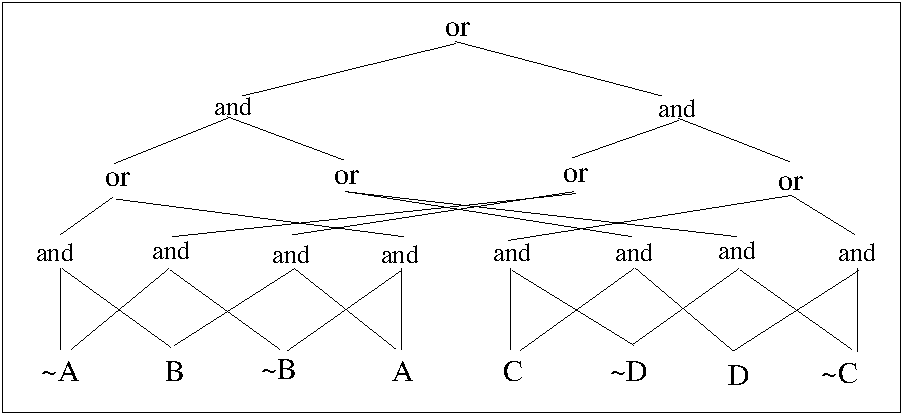
\includegraphics[width=8cm]{odd}
\caption{A decomposable and deterministic NNF.}
\label{fig:dnnf}
\end{figure}


\item[Query Rewriting Solutions] \mbox{}\\
A number of algorithms have been developed to find the rewritings of a given query; the most prominent being the bucket algorithm~\cite{levy:bucket},  the inverse rules algorithm ~\cite{duschka:answer,Qian96}, the minicon algorithm ~\cite{pottinger:minicon}, and the {\it MCDSat} ~\cite{arvelo:aaai06}. Generally, query rewriting algorithms work in two phases: first, they identify the views that rewrite at least one  subgoal of the query; second they combine the selected views to produce a rewriting. The main difference between existing approaches, is the criteria used to choose the relevant views and reduce the space of non-useful rewritings.

The bucket algorithm reduces the number of possibilities just considering each subgoal in the query in isolation, and selecting the views that are able to  produce at least the attributes projected by the query. Since, attributes involved in query joins are not verified, a large number of rewritings comprised of  Cartesian products may  be generated. 	
The Inverse Rules algorithm constructs a set of rules that invert the view definition and establish how to compute tuples for the database relations from tuples of the views. Similarly, to the bucket algorith it can produce a large number non-useful of rewritings. 

The MiniCon algorithm  overcomes the limitations of the previous algorithms by identifying only views that rewrite a set of the query goals and that  can be combined with the rest of the query subgoals. The key idea is to identify the mappings between  the variables in each subgoal of the query to the variables  in one or more subgoals of the views, in a way that, join variables in the query are mapped to join variables in the body of a view or to the distinguished variables of the view. Mappings between variables and subgoals are represented in MiniCon Descriptions (MCD's)\cite{pottinger:minicon}.

Finally,  the
{\it MCDSat} algorithm is able to identify the query rewritings of a query by translating the problem of rewriting
into the problem of enumerating the models of a propositional
theory  $\Theory{\Q}$ whose models are in correspondence
with the rewritings of the query. 
The {\it MCDSat} algorithm exploits the properties of d-DNNFs to efficiently 
compute the MCDs associated with theory $\Theory{\Q}$.
The  {\it MCDSat} algorithm has demonstrated to scale better than the MiniCon
algorithm over a large number of benchmarks often showing performance
improvements of several orders of magnitude. However, the McdSat algorithm was not desgined for rewriting problems involving explicit constants,
nor to compute the best rewritings with respect to a given utility function or cost model, and this paper we propose a new encoding  that overcomes these limitations.


\end{description}

\section{The McdSat$^c$ Architecture}

In order to do so, the theory $\Theory{\Q}$ is transformed into a d-DNNF
theory $\Delta(\Q)$ with a CNF to d-DNNF compiler.
The compiler's algorithm is similar to the DPLL algorithm
for SAT but enhanced with advanced techniques such as clause
learning and caching.
\begin{figure}
\centering
%COMENTADO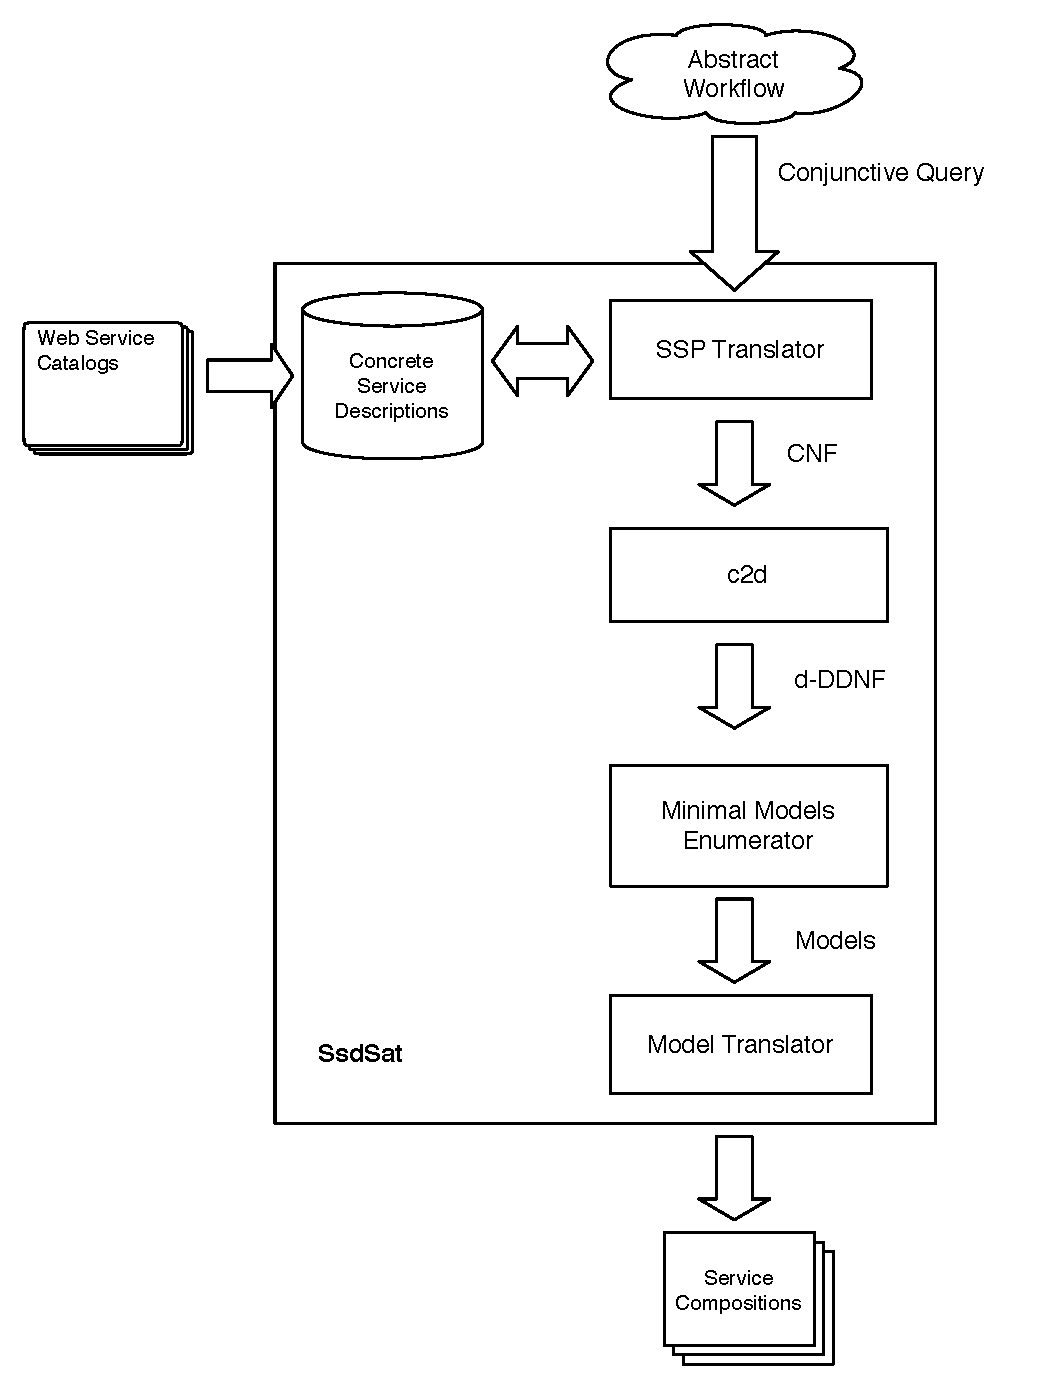
\includegraphics[width=10cm]{mdcsatC.pdf}
\caption{The McdSat$^c$ Architecture}
\label{fig:dnnf}
\end{figure}



\section{Experimental Results}
We have conducted an empirical analysis  on the benefits of the techniques implemented in the   McdSat$^c$ system.

\begin{description}
\item[Dataset and Query Benchmark:]  we conducted our experiments over a benchmark that includes XX queries and a set of  YY views. Queries and views are starts and chains, and they have between ZZ and fTT constants; queries have QQ sub-subgoals.
\item[Evaluation Metrics:] we report on runtime performance which corresponds to the  {\it user time} produced by the {\it time} command of the Unix operation system. 
\end{description}
 
\begin{figure}
\centering
%COMENTADO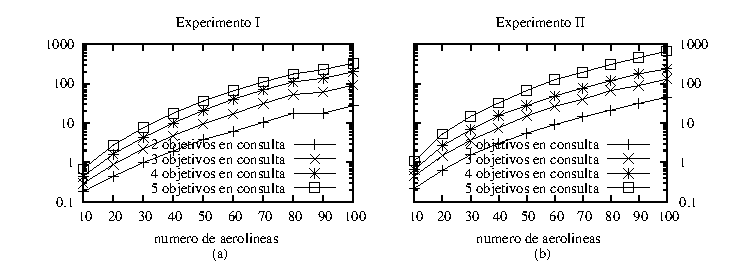
\includegraphics[width=8cm]{plot1.pdf}
\caption{Compilation Time Benchmark I}
\label{fig:plot1}
\end{figure}


\section{Formalization of the Service Selection Problem}

We consider databases of the form $D=\tup{P,T}$ where
$P$ is a set of predicates and $T=\{T_p\}_{p\in P}$ is a collection
of tables that represents the predicates in extensional form.
A conjunctive query $Q$ over $P$ is of the form 
\begin{alignat*}{1}
Q(\vvec{x})\ \qrule\ \  p_1(\vvec{x}_1),\, p_1(\vvec{x}_2),\, \ldots,\, p_m(\vvec{x}_m)\,,
\end{alignat*}
where $p_i\in P$, $\vvec{x}$ is a vector of variables, and each
$\vvec{x}_i$ is a vector of variables and constants.
The result of $Q$ over $D$, denoted as $Q(D)$, is the table with
$|\vvec{x}|$ columns that result of the projection of the relational
join $\join\!\!\{T_{p_i}\}_{i=1}^m$ over $\vvec{x}$.
The atoms in the body of $Q$ are called the (sub)goals of $Q$.

A view $V$ over $D$ is a query over $P$. In the context of the service selection problem, 
the database $D$ is an idealized description of 
the output produced abstract workflow  implemented by multiple concrete services described
as views.
Given a database $D$, a query $Q$ and a collection of 
views $E=\tup{\{V_i\}_i,\{E_i\}_i}$, we are required to find
all the tuples in $Q(D)$ obtainable from the views in $E$.
That is, we need to find all the \emph{compositions} of the form
\begin{alignat*}{1}
R(\vvec{x})\ \qrule\ \ V_{i_1}(\vvec{x}_1),\, V_{i_2}(\vvec{x}_2),\, \ldots,\, V_{i_n}(\vvec{x}_n)
\end{alignat*}
such that $R(E) \subseteq Q(D)$.
A service selection problem (SSP) is a tuple $\tup{P,Q,\{V_i\}}$ where $P$
is a set of predicates that represent abstract services, $Q$ is a query over $P$ and $\{V_i\}$ is a collection of views that define the concrete services in terms of  abstract services. We assume \emph{safe} problems in the sense that all 
variables mentioned in the head of the query (resp.\ in the head of each view)
appear in the body of the query (resp.,\ in the body of each view); also the input and output restrictions of the abstract services used in the query are satisfied.
Further, we only deal with SSPs with no arithmetic predicates inside the
query or views.
A composition $C$ is \emph{valid} if for all databases $D=\tup{P,T}$
and extensions $\{E_i\}$, $R(E) \subseteq Q(D)$.
A collection $\R$ of valid compositions is a solution if
for all databases $D=\tup{P,T}$ and extensions $\{E_i\}$, there
is no other $\R'$ such that $\R(E)\subset\R'(E)\subseteq Q(D)$.
We are interested in finding a composition $\R$.

\subsection{Logical Theories}

In \cite{arvelo:aaai06}, we showed that a rewriting
for a query $Q$ with $m$ goals can be obtained by enumerating the
models of a logical theory
$\Delta=\Delta_{rew}\cup\Delta_{mcd}^1\cup\cdots\Delta_{mcd}^m$
where $\Delta_{rew}$ specified how to combine $m$ independent
copies of MCD theories $\Delta_{mcd}$ that cover all goals in $Q$.
Each $\Delta^i_{mcd}$ is a copy of the theory $\Delta_{mcd}$
in which each literal $p$ is tagged as $p^i$.
The theory $\Delta_{mcd}$ consists of different groups of 
clauses that guarantees that its models are in correspondence
with the MCDs, while the theory $\Delta_{rew}$ contains additional
clauses to guarantee a sound and complete composition of the MCDs.
The reader is referred to \cite{arvelo:aaai06} for a comprehensive
description of the propositional theory.

Let us describe the difficulties that arise when constants
are presents in a SSP with the following example:
\begin{alignat*}{1}
Q(x,z)\ &\qrule\ \ p_1(x,y),\, p_2(y,z)\,, \\
V_1(x_1)\ &\qrule\ \ p_1(x_1,A)\,, \\
V_2(x_2)\ &\qrule\ \ p_2(B,x_2)\,, \\
V_3(x_3,y_3)\ &\qrule\ \ p_2(x_3,y_3)
%V_4(x_4,y_4)\ &\qrule\ \ p_1(x_1,A),\, p_2(B,y_4)\,,
\end{alignat*}
where $Q$ is the query and $\{V_1,V_2,V_3\}$ are the 
views. In this case, the only rewriting is 
$R(x,z)\qrule V_1(x),V_3(A,z)$ because the candidate 
$R(x,z)\qrule V_1(x),V_2(z)$ is not valid as it maps
$y$ into constants $A$ and $B$ that denote different
objects.

The main problem when handling constants is to
be sure that different constants are not mapped into
each other either directly or indirectly (via transitivity).

\subsection{Utility Functions}

We assume a simple additive utility function in which each view
$V_i$ is associated with a utility measure $c(V_i)$, and the overall utility value of
a composition is the sum of the utility values for the views in it.
An optimal or best service composition is one with maximum utility value,
and the optimal utility value of a SSP is the utility value of a best
service composition. A SSP has always a well-defined optimal
utility value (if there are no compositions, its utility is $0$),
but it may have multiple best service compositions.
The service composition problem with utility consists in finding
all the compositions of maximum utility value.

%The cost model is simple yet expressive; e.g., if all
%costs are unit, then best rewritings are those with
%minimum number of views, yet in cases where views
%represent different sources, it is natural
%to associate them with different costs.


\subsection{Extended Theories}

The theory $\Delta_{mcd}$ makes use of propositions $t_{x,y}$
to denote that the variable/constant $x$ in the query is mapped
into the variable/constant $y$ in the view, and propositions $v_i$
to indicate that the MCD uses view $V_i$.
We obtain a sound and complete theory for SSPs with constants if
$\Delta_{mcd}$ is extended with the clauses:

\begin{enumerate}[C1.]\denselist
\item (Inconsistent-1): $t_{x,A} \Rightarrow \neg t_{x,B}$,
\item (Inconsistent-2): $t_{A,x} \Rightarrow \neg t_{B,x}$,
\item (Inconsistent-3): $\neg t_{A,B}$,
\item (Transitivity-1): $v_i\land t_{A,y}\land t_{x,y}\land t_{x,z}\Rightarrow t_{A,z}$,
\item (Transitivity-2): $v_i\land t_{y,A}\land t_{y,x}\land t_{z,x}\Rightarrow t_{z,A}$.
\end{enumerate}
Clauses C1--C3 prune candidate service compositions in which one constant
is directly mapped into a different one, and the last two implement
a restricted propagation of transitivity.
Similarly, $\Delta_{rew}$ must be extended with the clauses:
\begin{enumerate}[C1.]\denselist
\item[C6.] (Inconsistent-4): $t^i_{x,A} \Rightarrow \neg t^j_{x,B}$.
\end{enumerate}
~\cite{RajaramanSU95} showed that for queries without negation or arithmetic comparisons,  but with constants, and $m$ goals and $q$ variables, it is enough
to consider service compositions of length at most  $m$ plus  $q$ subgoals ~\cite{Ullman00}.

Given a SSP problem $\tup{Q,\{V_i\}}$ possibly with constant 
symbols, we construct logical theories whose models are in
correspondence with the service compositions. These theories are then
compiled into d-DNNF from which all rewritings are extracted
efficiently.
Likewise, best service compositions can be computed by performing model
enumeration twice: the first pass computes the optimal utility function,
and the second filters out suboptimal service compositions.
However, there is a better way, which we will describe in the next section.

\subsection{Maximum-Utility Function}

Darwiche \& Marquis \cite{darwiche:weighted} show how to compute the
rank $r^*(\Delta)$ of a propositional theory $\Delta$
efficiently when $r$ is a literal ranking function and
$\Delta$ is in d-DNNF. A literal ranking function ranks
the models of the theory in terms of the rank of the
literals $l$ that are true in the model, and ranks the
theory as the best rank of its models:
\[ r(\omega) = \sum_{\omega\vDash l} r(l),\quad r^*(\Delta) = \max_{\omega\vDash\Delta} r(\omega)\,. \]
Furthermore, not only $r^*(\Delta)$ can be computed
efficiently from the d-DNNF but also the models that
have such rank.
The procedure for computing the rank converts the d-DNNF
into a circuit in which the literals are replaced by their
ranks, the `or' nodes by `max', and the `and' nodes by `sum'.
The evaluation of the circuit computes the rank of $\Delta$.

We thus obtain a simple method for computing the best
rewritings when the literal ranking function $r_c$ induced
by the cost model $c$ is used; $r_c$ is defined by
$r_c(l)=c(V_i)$ if $l=v^t_i$ for some $t$, and $r_c(l)=0$
otherwise.


\section{Conclusions and Future Work}

compute the best rewritings with respect to an additive
cost model. The cost model is simple yet expressive.
The computation of the best models relies on an arithmetic
circuit that is obtained from the d-DNNF of the propositional
theory.
}

%%%%%%%%%%%%%%%%%%%%%%%%%%%%%%%%%%%%%%%%%%%%%%%%%%%%%%%%%%%%%%%%%%%%%%%%%%%%%%%%
%%%%%%%%%%%%%%%%%%%%%%%%%%%%%%%%%%%%%%%%%%%%%%%%%%%%%%%%%%%%%%%%%%%%%%%%%%%%%%%%
%TODO
%en la parte del cuadro de Servicios Abstractos y Concretos sale cuadro 1 pero
%el label dice cuadro 2
%%%%%%%%%%%%%%%%%%%%%%%%%%%%%%%%%%%%%%%%%%%%%%%%%%%%%%%%%%%%%%%%%%%%%%%%%%%%%%%%
%%%%%%%%%%%%%%%%%%%%%%%%%%%%%%%%%%%%%%%%%%%%%%%%%%%%%%%%%%%%%%%%%%%%%%%%%%%%%%%%

\begin{titlepage}

\begin{flushleft}

\includegraphics[scale=0.3]{graphics/logo_usb.png} \\
Universidad Simón Bolívar \\
Coordinación de Ciencias de la Computación \\
Maestría en Ciencias de la Computación \\
\end{flushleft}

\vspace{0.8cm}

\begin{center}
{\large \bf \textsf{Instanciación Óptima de Flujos de Trabajo Abstractos Usando Lógica y Circuitos}}
\end{center}

\vspace{0.2cm}

\begin{abstract}
Una arquitectura orientada a servicios típica se separa en dos capas --grupos de
componentes-- principales.
La capa concreta con servicios concretos cuyas funcionalidades son descritas en
términos de pre- y post-condiciones y propiedades no funcionales en términos de
parámetros de calidad de servicio (Quality Of Service, QoS), y la capa abstracta
con aplicaciones de software cuyas funcionalidades son descritas en términos de
flujos de trabajo abstractos y propiedades no funcionales en términos de
restricciones sobre QoS. Durante la ejecución de un flujo de trabajo o \emph{workflow}, los
servicios abstractos son instanciados en servicios concretos que cumplen con los
requerimientos funcionales y no funcionales. Esta instanciación, que debe ser
hecha en el momento, consiste de una búsqueda en un espacio de posibilidades
combinatorio. En este trabajo se propone una infraestructura para resolver
eficientemente el problema de instanciación que está basada en
la lógica proposicional. La infraestructura adopta el enfoque de definición denominado Local-As-View en la cual la
funcionalidad de servicios concretos se describe usando vistas de servicios
abstractos, la calidad de una instanciación como una función de utilidad global
que combina los diferentes parámetros QoS, y los flujos de trabajo abstractos
como consultas conjuntivas sobre servicios abstractos. Usando esta
representación, el problema de instanciación de flujos de trabajo se convierte
en un problema de reescritura de consultas, del área de sistemas de integración.
Entonces, en base a enfoques reportados en la literatura, se propone una codificación del
problema de instanciación de flujos de trabajo como una teoría lógica cuyos
modelos están en correspondencia con las instanciaciones del flujo de trabajo, y
los modelos mejor calificados en correspondencia con instanciaciones óptimas del
flujo de trabajo. Así, explotando propiedades conocidas de teorías lógicas en
formato d-DNNF, se provee una solución eficiente y escalable al problema de
instanciación de flujos de trabajo. Esta solución no sólo escala a
instancias grandes como muestran resultados experimentales ya realizados, sino
que también podemos verificar que es correcta y completa dado que, estando basada en la lógica, es
fácilmente sujeta al análisis formal.
\end{abstract}

\vspace{\fill}

\begin{minipage}{0.3\textwidth}
\begin{flushleft}
\emph{Estudiante:} \\
Daniel \textsc{Izquierdo} \\
Carnet 08-86809 \\
\end{flushleft}
\end{minipage}
\begin{minipage}{0.3\textwidth}
\begin{center}
Fecha estimada de culminación: \\
Marzo de 2010
\end{center}
\end{minipage}
\begin{minipage}{0.3\textwidth}
\begin{flushright}
\emph{Asesores:} \\
Prof. Blai \textsc{Bonet} \\
Prof. María Esther \textsc{Vidal} \\
\end{flushright}
\end{minipage}

\end{titlepage}


\tableofcontents
\newpage

\section{Planteamiento del Problema}

En el contexto de la Web Semántica, y con el soporte de las Arquitecturas Orientadas a
Servicios (SOA), el número de fuentes de datos y servicios Web ha explotado en
los últimos años. Por ejemplo, la colección de bases de datos de biología
molecular actualmente contiene 1.170 bases de datos~\cite{Galperin09}, un número
que es
mayor que el del último año por 95~\cite{Galperin2008}, y que el de hace dos
años por 110~\cite{Galperin2007};
las herramientas y servicios, así como el número de instancias
publicados por estos recursos, siguen una progresión similar~\cite{Benson07}.
Gracias a
esta variedad de datos, la tendencia de los usuarios es hacia depender cada vez
más de métodos automáticos para manejarlos tales como recuperación de datos de
fuentes públicas y análisis utilizando herramientas o servicios Web compuestos
en flujos de trabajo complejos.

La SOA típica consiste de dos capas. La capa concreta que está hecha de
servicios concretos cuyas funcionalidades son descritas en términos de pre- y
post-condiciones y propiedades no funcionales en conjuntos de parámetros de
calidad de servicio (QoS), y
la capa abstracta compuesta de aplicaciones de software cuyas funcionalidades
son descritas en términos de flujos de trabajo abstractos y propiedades no
funcionales en términos de restricciones de QoS. La ejecución de un flujo de
trabajo abstracto involucra la instanciación de los servicios abstractos en
servicios concretos que cumplan con los requerimientos funcionales y no
funcionales. Este proceso de instanciación puede ser visto como una búsqueda de
una instanciación objetivo en el espacio combinatorio de todas las
instanciaciones válidas. Entonces se está interesado en técnicas eficientes para
realizar esta búsqueda que sean capaces de escalar a medida que el número de
servicios concretos o la complejidad (número
de objetivos, tamaño) de la estructura del flujo de trabajo  aumenta. Se llama al
problema de instanciar un flujo de trabajo dado con servicios concretos de un
conjunto de servicios concretos dado, de manera que ciertas restricciones sobre QoS sean
cumplidas, el Problema de Instanciación de Flujos de Trabajo (WIP).

En este trabajo se considera una versión restringida de WIP que adopta el
enfoque Local-As-View (LAV) \cite{levy:bucket}. En LAV, todos los elementos de un
problema son especificados con un lenguaje común basado en servicios abstractos
tal que los servicios concretos se describen como vistas de servicios
abstractos, la calidad de una instanciación como una función de utilidad global
que combina los diferentes parámetros QoS, y el flujo de trabajo abstracto como
una consulta conjuntiva sobre los servicios abstractos; esta representación es
similar a la que es generada de manera semiautomática para el sistema DEIMOS
\cite{AmbiteISWC09}. En esta versión de WIP, las reglas que definen flujos de trabajo
(consultas conjuntivas) y servicios concretos (vistas) son creados de manera que
todas las restricciones funcionales sobre pre- y post-condiciones de los
servicios y sus combinaciones sean satisfechas, y las medidas de QoS son
representadas anotando cada descripción de servicio concreto con un número real
que representa la utilidad QoS global del servicio.

Bajo estas suposiciones, WIP puede ser convertido en el bien conocido Problema
de Reescritura de Consultas (QRP) para LAV que es central a los sistemas de
integración \cite{halevy:survey}. QRP consiste de una consulta conjuntiva que debe ser
respondida en términos de vistas donde la consulta y las vistas son descritas
usando LAV con relaciones abstractas. Este problema es importante en el contexto
de integración de datos \cite{Chen05,JaudoinPRST05}, y optimización de consultas y mantenimiento
de datos \cite{AfratiLU07,levy:bucket}, y varias soluciones que escalan a un número grande de
vistas han sido definidas \cite{arvelo:aaai06,pods:DuschkaG97,sac:DuschkaG97,levy:bucket,pottinger:minicon}.

La solución propuesta por Arvelo et al. \cite{arvelo:aaai06} está basada en la enumeración
eficiente de modelos de una teoría lógica proposicional. Dada una consulta conjuntiva
y un conjunto de fuentes definidas como vistas, se construye una teoría
lógica de manera que cada modelo de la teoría codifica una
reescritura válida, y así todas las reescrituras son obtenidas enumerando los
modelos de la teoría. Esta enumeración puede ser realizada eficientemente si la
teoría lógica está en cierta forma normal llamada la forma normal de negación
determinística y descomponible (d-DNNF) \cite{darwiche:d-dnnfs}. Así,
la solución consiste en transformar (llamado compilar en el campo de
compilación del conocimiento) la teoría lógica en el formato d-DNNF para
enumerar sus modelos eficientemente.

Pero las teorías d-DNNF no sólo soportan la enumeración eficiente de sus
modelos, sino también otras operaciones. Entre ellas se encuentra la enumeración
de los modelos con mejor calidad. Dada una función de calidad de literales
$r(\ell)$ que asigne calidades a cada literal $\ell$, se define la calidad
$r(\omega)$ de un modelo $\omega$ como la suma de las calidades de los literales
activados por $\omega$ (es decir,
$r(\omega)\doteq\sum_{\omega\vDash\ell}r(\ell)$), y se dice que $\omega$ es un modelo
de mejor calidad si no hay modelo $\omega'$ tal que $r(\omega')<r(\omega)$.

Dada una teoría en d-DNNF, se computa la calidad de los mejores modelos, y
los mejores modelos, en tiempo lineal en el tamaño del d-DNNF. Este cómputo
transforma el GAD del d-DNNF en un circuito aritmético reemplazando los nodos
AND con `+' y los nodos OR con `min'. La función de calidad de literales
asigna valores a las hojas del circuito aritmético (grafo acíclico dirigido usado
para calcular polinomios) que son propagados a la raíz en tiempo
lineal. El valor de la raíz es la calidad del mejor modelo \cite{darwiche:weighted}.

En este trabajo se propone explotar las propiedades de los d-DNNF construyendo una
teoría lógica cuyos modelos codifican las instanciaciones del flujo de trabajo
y cuyos mejores modelos codifican las instanciaciones óptimas (mejores). Así, la
búsqueda combinatoria se reduce a la computación de un mejor modelo de una
teoría lógica que puede ser realizada eficientemente una vez que la teoría es
transformada al formato d-DNNF.

\subsection{Ejemplo Motivante}

% flights
\newcommand{\vuelo}{\text{\it vuelo}}
\newcommand{\ciudadVE}{\text{\it ciudadVE}}
\newcommand{\nacional}{\text{\it nacional}}
\newcommand{\ida}{\text{\it ida}}
\newcommand{\unaescala}{\text{\it una-escala}}
\newcommand{\vueloCCS}{\text{\it vuelo-hacia-ccs}}
\newcommand{\unaparadaCCS}{\text{\it unaescala-hacia-ccs}}
\newcommand{\desdeVAL}{\text{\it desde-val}}
\newcommand{\PA}{\text{CCS}}
\newcommand{\NY}{\text{VAL}}
\newcommand{\AL}{\text{AL}}
% end flights

Considere un sistema simple de información de vuelos que contiene información
sobre vuelos entre ciudades e información sobre qué ciudades están en los
Estados Unidos. Un sistema así puede ser descrito usando LAV con los dos servicios
abstractos $\vuelo(x,y)$ y $\ciudadVE(x)$. El primero relaciona dos ciudades $x$ e $y$ si
hay un vuelo directo entre ellas, y el segundo dice si $x$ es una ciudad de
Venezuela  o no. Para los servicios concretos, supongamos que las fuentes de
datos disponibles en Internet contienen la siguiente información:

\begin{enumerate}[--]
\item $\nacional(x,y)$ relaciona dos ciudades de Venezuela conectadas por un vuelo directo,
\item $\ida(x,y)$ relaciona dos ciudades conectadas por un vuelo de ida,
\item $\unaescala(x,y)$ relaciona dos ciudades conectadas por un vuelo con una escala,
\item $\vueloCCS(x)$ dice si hay un vuelo directo desde $x$ a Caracas,
\item $\unaparadaCCS(x,y)$ relaciona $x$ y $y$ si hay un vuelo desde $x$ a Caracas con una escala en $y$, y
\item $\desdeVAL(x)$ dice si hay un vuelo de Valencia a $x$.
\end{enumerate}

Adicionalmente, los servicios concretos se describen con los siguientes
servicios abstractos:

\begin{alignat*}{1}
\nacional(x,y)\   &\qrule\ \vuelo(x,y),\,\ciudadVE(x),\,\ciudadVE(y)\,. \\
\ida(x,y)\     &\qrule\ \vuelo(x,y)\,. \\
\unaescala(x,z)\    &\qrule\ \vuelo(x,y),\,\vuelo(y,z)\,. \\
\vueloCCS(x)\     &\qrule\ \vuelo(x,\PA)\,. \\
\unaparadaCCS(x,y)\  &\qrule\ \vuelo(x,y),\,\vuelo(y,\PA)\,. \\
\desdeVAL(x)\       &\qrule\ \vuelo(\NY,x)\,.
\end{alignat*}

Ahora supongamos que un usuario está interesado en construir una aplicación
capaz de recuperar los vuelos ida y vuelta con una parada hacia cualquier ciudad
en el mundo, tales que los vuelos puedan detenerse en cualquier ciudad.

\[ W(x,w,y,z) \qrule \ciudadVE(x),\,\vuelo(x,w),\,\vuelo(w,y),\,\vuelo(y,z),\,\vuelo(z,x)\,. \]

La siguiente consulta conjuntiva representa el flujo de trabajo que define esta
solicitud en términos de servicios abstractos. El flujo de trabajo es definido
de manera que todo lo relacionado sobre el ligamiento de parámetros de
entrada/salida es resuelto. Así, cualquier instanciación de los servicios
abstractos en términos de los servicios concretos es una implementación válida
del flujo de trabajo. Las implementaciones corresponden a composiciones de
servicios concretos en las cuales un servicio concreto puede implementar uno o
más servicios abstractos del flujo, pero cada servicio abstracto puede ser
implementado por exactamente un servicio concreto. Por ejemplo, la siguiente
composición corresponde a una de estas implementaciones.

\[ I(x,w,y,z)\ \qrule\ \nacional(x,w),\,\vueloCCS(w),\,\ida(\PA,z),\,\nacional(z,x)\,. \]

Sin embargo, las siguientes dos composiciones no son válidas.

\begin{alignat*}{1}
I'(x,w,y,z)\  \qrule\ &\nacional(x,y),\,\vueloCCS(y),\,\desdeVAL(z),\,\nacional(z,x)\,. \\
I''(x,w,y,z)\ \qrule\ &\unaescala(x,y),\,\ida(y,z),\,\nacional(z,x)\,.
\end{alignat*}

La primera composición no es válida porque asocia la variable del flujo $y$ a
las constantes \PA\ y \NY\ que denotan ciudades diferentes. En la otra mano, $I''$
no lo implementa porque el servicio concreto $\unaescala(x,y)$ no recibe como entrada
o produce como salida la ciudad intermedia donde el vuelo se detiene y entonces
no es posible asegurarse de que esa ciudad esté asociada a la ciudad $w$ que es
retornada por el flujo de trabajo.

Estos ejemplos muestran que las instanciaciones correctas de un flujo deben
manejar constantes de manera que dos constantes distintas no sean asociadas
entre sí de manera directa o indirectamente vía transitividad, y que todos los
atributos que aparezcan en un \emph{join} o en la salida sean producidos por los
servicios concretos seleccionados.

Los parámetros QoS son modelados anotando los servicios concretos con utilidades
que caracterizan su comportamiento y que luego son agregados durante la
instanciación. Así, como se mencionó previamente, la mejor instanciación es la
que minimiza (o maximiza) la agregación de utilidades.

\section{Justificación e importancia}

\subsection{Ejemplo motivante}

% flights
\newcommand{\flight}{\text{\it flight}}
\newcommand{\UScity}{\text{\it uscity}}
\newcommand{\national}{\text{\it national}}
\newcommand{\oneway}{\text{\it one-way}}
\newcommand{\onestop}{\text{\it one-stop}}
\newcommand{\flightPA}{\text{\it flight-to-pa}}
\newcommand{\onestopPA}{\text{\it onestop-to-pa}}
\newcommand{\fromNY}{\text{\it from-ny}}
\newcommand{\PA}{\text{PA}}
\newcommand{\NY}{\text{NY}}
\newcommand{\AL}{\text{AL}}
% end flights

Considere un sistema simple de información de vuelos que contiene información
sobre vuelos entre ciudades e información sobre qué ciudades están en los
Estados Unidos. Un sistema así puede ser descrito usando LAV con los dos servicios
abstractos $\flight(x,y)$ y $\UScity(x)$. El primero relaciona dos ciudades $x$ e $y$ si
hay un vuelo directo entre ellas, y el segundo dice si $x$ es una ciudad de
E.E.U.U.  o no. Para los servicios concretos, supongamos que las fuentes de
datos disponibles en Internet contienen la siguiente información:

\begin{enumerate}[--]
\item $\national(x,y)$ relaciona dos ciudades de E.E.U.U. conectadas por un vuelo directo,
\item $\oneway(x,y)$ relaciona dos ciudades conectadas por un vuelo de ida,
\item $\onestop(x,y)$ relaciona dos ciudades conectadas por un vuelo con una escala,
\item $\flightPA(x)$ dice si hay un vuelo directo desde $x$ a París,
\item $\onestopPA(x,y)$ relaciona $x$ y $y$ si hay un vuelo desde $x$ a París con una escala en $y$, y
\item $\fromNY(x)$ dice si hay un vuelo de Nueva York a $x$.
\end{enumerate}

Adicionalmente, los servicios concretos se describen con los siguientes
servicios abstractos:

\begin{alignat*}{1}
\national(x,y)\   &\qrule\ \flight(x,y),\,\UScity(x),\,\UScity(y)\,. \\
\oneway(x,y)\     &\qrule\ \flight(x,y)\,. \\
\onestop(x,z)\    &\qrule\ \flight(x,y),\,\flight(y,z)\,. \\
\flightPA(x)\     &\qrule\ \flight(x,\PA)\,. \\
\onestopPA(x,y)\  &\qrule\ \flight(x,y),\,\flight(y,\PA)\,. \\
\fromNY(x)\       &\qrule\ \flight(\NY,x)\,.
\end{alignat*}

Ahora supongamos que un usuario está interesado en construir un flujo de trabajo
capaz de recuperar los vuelos ida y vuelta con una parada hacia cualquier ciudad
en el mundo, tales que los vuelos puedan detenerse en cualquier ciudad.

\[ W(x,w,y,z) \qrule \UScity(x),\,\flight(x,w),\,\flight(w,y),\,\flight(y,z),\,\flight(z,x)\,. \]

La siguiente consulta conjuntiva representa el flujo de trabajo que define esta
solicitud en términos de servicios abstractos. El flujo de trabajo es definido
de manera que todo lo relacionado sobre el ligamiento de parámetros de
entrada/salida es resuelto. Así, cualquier instanciación de los servicios
abstractos en términos de los servicios concretos es una implementación válida
del flujo de trabajo. Las implementaciones corresponden a composiciones de
servicios concretos en las cuales un servicio concreto puede implementar uno o
más servicios abstractos del flujo, pero cada servicio abstracto puede ser
implementado por exactamente un servicio concreto. Por ejemplo, la siguiente
composición corresponde a una de estas implementaciones.

\[ I(x,w,y,z)\ \qrule\ \national(x,w),\,\flightPA(w),\,\oneway(\PA,z),\,\national(z,x)\,. \]

Sin embargo, las siguientes dos composiciones no son válidas.

\begin{alignat*}{1}
I'(x,w,y,z)\  \qrule\ &\national(x,y),\,\flightPA(y),\,\fromNY(z),\,\national(z,x)\,. \\
I''(x,w,y,z)\ \qrule\ &\onestop(x,y),\,\oneway(y,z),\,\national(z,x)\,.
\end{alignat*}

La primera composición no es válida porque asocia la variable del flujo $y$ a
las constantes \PA\ y \NY\ que denotan ciudades diferentes. En la otra mano, $I''$
no lo implementa porque el servicio concreto $\onestop(x,y)$ no recibe como entrada
o produce como salida la ciudad intermedia donde el vuelo se detiene y entonces
no es posible asegurarse de que esa ciudad esté asociada a la ciudad $w$ que es
retornada por el flujo de trabajo.

Estos ejemplos muestran que las instanciaciones correctas de un flujo deben
manejar constantes de manera que dos constantes distintas no sean asociadas
entre sí de manera directa o indirectamente vía transitividad, y que todos los
atributos que aparezcan en un \emph{join} o en la salida sean producidos por los
servicios concretos seleccionados.

Los parámetros QoS son modelados anotando los servicios concretos con utilidades
que caracterizan su comportamiento y que luego son agregados durante la
instanciación. Así, como se mencionó previamente, la mejor instanciación es la
que minimiza (o maximiza) la agregación de utilidades.


\section{Objetivos}

\begin{enumerate}
\item Desarrollar un sistema capaz de resolver instancias WIP con constantes y
costos que escale a tamaños razonables.
\item Desarrollar un sistema capaz de resolver instancias WIP muy grandes con
constantes y costos en tiempo razonable.
\item Dar al sistema desarollado la capacidad de manejar clases de constantes.
\end{enumerate}

\section{Metodología Propuesta}

La fase inicial de este trabajo consiste en realizar una investigación sobre el
problema a ser tratado. Se debe conocer el estado del arte en cuanto a resultados obtenidos
relacionados al problema y las líneas de investigación que se están siguiendo.

Una vez conocidas las propuestas actuales se procede a identificar sus
fortalezas y especialmente sus limitaciones. Se analizarán las causas de
dichas limitaciones y se propondrán maneras de superarlas. Las propuestas deben
estar acompañadas de un basamento formal que permita demostrar su correctitud y
deben ser implementables en un lapso razonable de manera de evaluar su
rendimiento y su capacidad de resolver el problema.

Luego comenzará la implementación de la nueva solución. Para ello se podrá
utilizar como punto de partida sistemas existentes como el propuesto por Arvelo
et al. \cite{arvelo:aaai06} y modificarlos para mejorar
sus características siguiendo las ideas propuestas.

La finalización del proceso de implementación dará paso a la fase de evaluación de
la propuesta. Se propone realizar series de experimentos diversos sobre el
producto final que ilustren sus capacidades y rendimiento. En casos en
que soluciones ya existentes tengan las mismas capacidades, se debe comparar el
rendimiento de ambas sobre una variedad de casos de prueba que persigan revelar
sus peores comportamientos. Esto permitirá determinar empíricamente las virtudes
y desventajas de la solución propuesta.

\section{Cronograma de Actividades}

\begin{tabular}{|p{8cm}|c|c|}
\hline
Actividad & Duración & Fecha estimada \\
\hline
\hline
Investigación sobre el estado del arte & 2 semanas & 2 de octubre de 2009\\
\hline
Identificación de limitaciones de propuestas actuales & 2 semanas & 16 de octubre de 2009\\
\hline
Propuesta de formalización del problema incluyendo manejo de constantes y costos & 2 semanas & 30 de octubre de 2009 \\
\hline
Pruebas formales sobre nueva formalización & 2 semanas &  13 de noviembre de 2009 \\
\hline
Implementación de generación de cláusulas nuevas para constantes & 2 semanas & 27 de noviembre de 2009 \\
\hline
Experimentos con generación de cláusulas nuevas & 3 semanas & 18 de diciembre de 2009 \\
\hline
Implementación de búsqueda de mejor reescritura & 2 semanas & 8 de enero de 2010 \\
\hline
Experimentos con búsqueda de mejor reescritura & 2 semana & 22 de enero de 2010 \\
\hline
Implementación de sistema para problemas de tamaño mayor & 5 semanas & 26 de febrero de 2010 \\
\hline
Experimentos de sistema para problemas de tamaño mayor & 3 semanas & 19 de marzo de 2010 \\
\hline
Implementación de soporte para clases de constantes & 2 semanas & 2 de abril de 2010 \\
\hline
Pruebas de soporte para clases de constantes & 2 semana & 16 de abril de 2010 \\
\hline
\end{tabular}


\addcontentsline{toc}{section}{Referencias} 
\bibliographystyle{abbrv}
\bibliography{ref}

\end{document}
